\chapter{I-Mode Pedestal Scalings}\label{ch:ImodePedestal}

The I-mode \cite{Whyte2010,Hubbard2011}, introduced in \cref{sec:hcr_imode}, is a novel high-performance regime pioneered on Alcator C-Mod.  I-mode is unique in that it appears to decouple energy and particle transport, forming a steep temperature pedestal with H-mode levels of energy confinement without the accompanying density pedestal or suppression of particle transport found in conventional H-modes.  I-mode exhibits several highly attractive properties for a putative reactor regime:

\begin{enumerate}
 \item Due to the lack of particle transport suppression (as is found in H-modes), the I-mode retains L-mode-like impurity confinement times, avoiding the accumulation of deleterious impurities in the plasma, including those from high-$Z$ metal plasma-facing components necessary for reactor operation \cite{Loarte2007}\gnote{check cite}.  This ensures stationary operation without the need for ELMs or continuous fluctuations in the edge to provide the necessary relaxation of the particle confinement.
 \item I-mode appears to be naturally stable against large ELMs, avoiding excessive pulsed heat loading to plasma-facing components without externally-applied engineering controls (described in \cref{subsec:hcr_elmy_control}).
 \item Energy confinement in I-mode appears to exhibit little to know degradation with input heating power, in contrast to that found in ELMy H-mode ($\tau_E \sim P^{-0.7}$ from the ITER98y2 analysis \cite{ITER1999}), scaling quite favorably to reactor-scale devices.
\end{enumerate}



\section{Access and Experimental Setup}\label{sec:imode_setup}

\nicesectionending

\section{Pedestal Responses}\label{sec:imode_height}

\subsection{Pedestal Response to Fueling}\label{subsec:imode_fueling}

\begin{figure}
 \pushtooutside
 \fcapside[60mm]{\caption[Density and temperature pedestals at matched current and field with varying fueling and heating power -- matched $P_{net}/\overline{n}_e$ maintains the $T_e$ pedestal.]{Density and temperature pedestals at matched current, field, and shaping, with varying fueling and heating power levels.  The three discharges are fueled to $\overline{n}_e$ of $\num{1.0}$ (black), $\num{1.3}$ (blue), and $\SI{1.7e20}{\per\meter\cubed}$ (red) respectively, with heating powers of $\num{2.75}$, $\num{3.65}$, and $\SI{4.10}{\mega\watt}$ to maintain matched $P_{net}/\overline{n}_e \sim 2.4-2.7$.  The constant power-per-particle maintains matched temperature pedestals across the fueling range, indicative of the independent control of pedestal $n_e$ and $T_e$ available in I-mode.}\label{fig:imode_fuelingprofiles}}{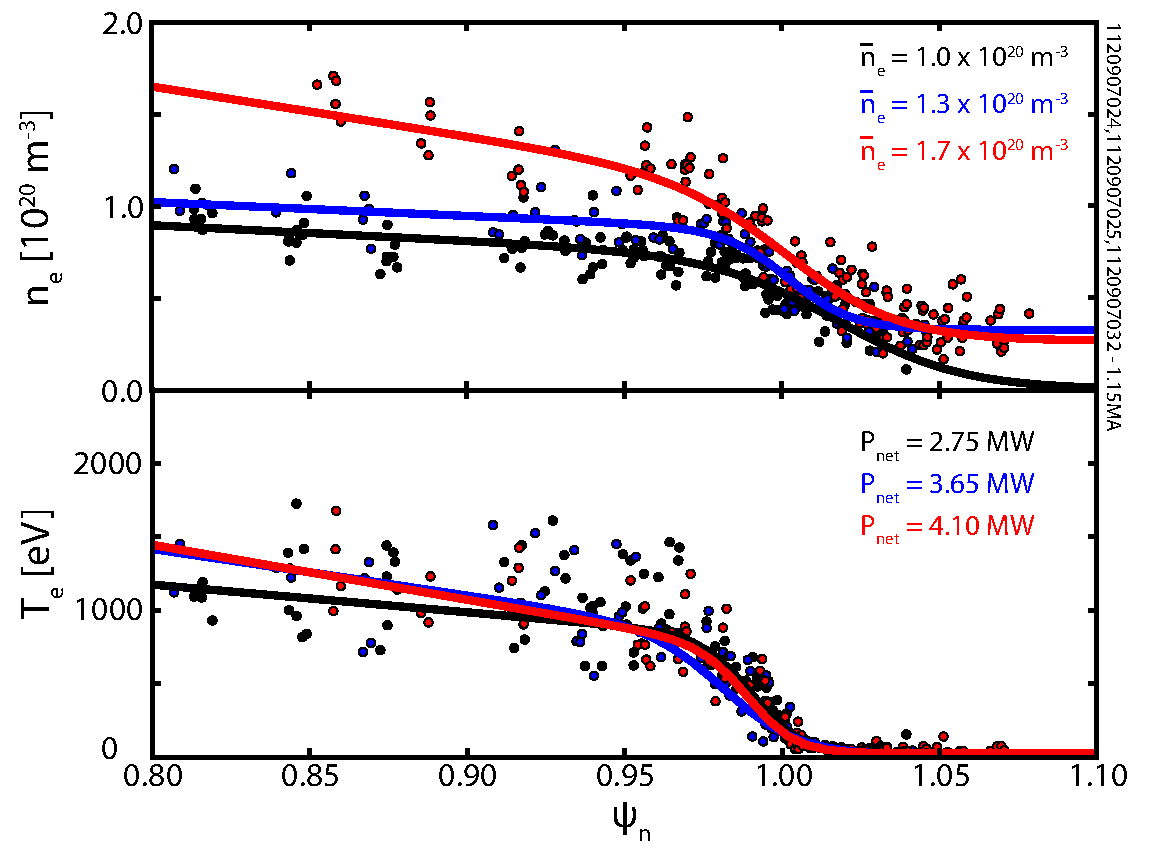
\includegraphics[width=100mm]{graphics/IModePedestal/fuelingprofiles.pdf}}
\end{figure}

\subsection{Pedestal Temperature}\label{subsec:imode_temp}

\subsection{Pressure Pedestal Scalings and Performance}\label{subsec:imode_pres}

\nicesectionending

\section{Pedestal Widths}\label{sec:imode_width}

\nicesectionending

\section{Global Behavior, Performance, \& Confinement}\label{sec:imode_confinement}

\begin{table*}
 \pushtooutside
 \ttabbox{\caption[Parameters for power-law scalings of I-mode energy confinement time.]{Parameters for power-law scalings of the I-mode energy confinement time $\tau_E$, along with $R^2$ coefficients of determination for the fit.  Blank entries indicate parameters that were omitted from that fit.  Note that fit \#5 utilized a fixed $R^2 \sqrt{\varepsilon}$ size dependence rather than taking the size to be a free fitting parameter.  Parameters are in the given units: $I_p$ in $\si{\mega\ampere}$, $B_T$ in $\si{\tesla}$, $\overline{n}_e$ in $\SI{e20}{\per\meter\cubed}$, $R$ in $\si{\meter}$, and $P_{loss}$ in $\si{\mega\watt}$.  Elongation $\kappa$ and aspect ratio $\varepsilon$ are dimensionless.}\label{tab:imode_confinement}}{
 \begin{tabular}{cccccc}
  \toprule
  & \#1 & \#2 & \#3 & \#4 & \#5 \\
  \midrule
  $C$ & $0.040 \pm 0.066$ & $0.007 \pm 0.002$ & $0.014 \pm 0.002$ & $0.014 \pm 0.002$ & $0.056 \pm 0.008$ \\
  $I_p$ & $0.686 \pm 0.074$ & $0.696 \pm 0.073$ & $0.685 \pm 0.076$ & $0.692 \pm 0.073$ & $0.676 \pm 0.077$ \\
  $B_T$ & $0.698 \pm 0.075$ & $0.697 \pm 0.071$ & $0.768 \pm 0.072$ & $0.773 \pm 0.071$ & $0.767 \pm 0.072$ \\
  $\overline{n}_e$ & $-0.077 \pm 0.055$ & $-0.050 \pm 0.048$ & $0.017 \pm 0.048$ & & $0.006 \pm 0.048$ \\
  $R$ & $4.219 \pm 4.623$ & & & & $2^*$ \\
  $\varepsilon$ & $0.127 \pm 1.144$ & & & & $0.5^*$ \\
  $\kappa$ & $1.686 \pm 0.398$ & $1.501 \pm 0.350$ & & & \\
  $P_{loss}$ & $-0.197 \pm 0.048$ & $-0.220 \pm 0.043$ & $-0.286 \pm 0.042$ & $-0.281 \pm 0.039$ & $-0.275 \pm 0.042$ \\
  $R^2$ & $0.713$ & $0.711$ & $0.685$ & $0.684$ & $0.683$ \\
  \bottomrule
 \end{tabular}
 }
\end{table*}

\begin{figure}
 \pushtooutside
 \fcapside[60mm]{\caption[Power-law fit to I-mode $\tau_E$ with full parameter set.]{Power-law fit for I-mode energy confinement time $\tau_E$, fitted using the full ITER98y2 parameter set (fit \#1 in \cref{tab:imode_confinement}).  Both the high-resolution pedestal database and older reversed-field LSN and forward-field USN I-mode databases are used.  While the fit is generally good, lack of variation in certain parameters -- particularly the size parameters $R$ and $\varepsilon$ (as expected for a single-machine scaling), and elongation $\kappa$ mean that the true variation with these parameters is not accurately captured.  However, the expected weak degradation of $\tau_E$ with heating power is captured.}\label{fig:imode_tauE_1}}{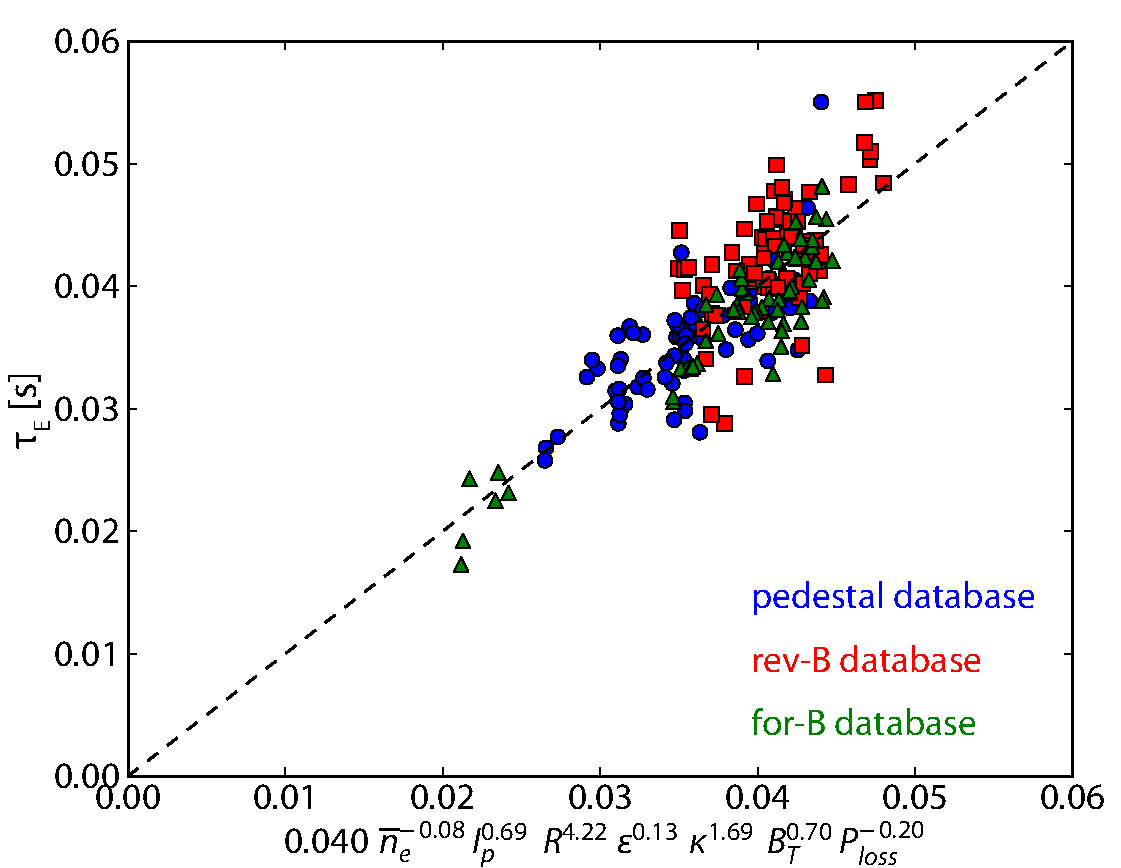
\includegraphics[width=100mm]{graphics/IModePedestal/tauE_1_Ploss_sep.pdf}}
\end{figure}

\begin{figure}
 \pushtooutside
 \fcapside[60mm]{\caption[Power-law fit to I-mode $\tau_E$, with poorly-fitted parameters excluded.]{Power-law fit for I-mode energy confinement time $\tau_E$, fitted with the size parameters $R$ and $\varepsilon$, and elongation $\kappa$ excluded due to the lack of variation in these variables in the available data (fit \#3 in \cref{tab:imode_confinement}).  Both the high-resolution pedestal database and older reversed-field LSN and forward-field USN I-mode databases are used.}\label{fig:imode_tauE_3}}{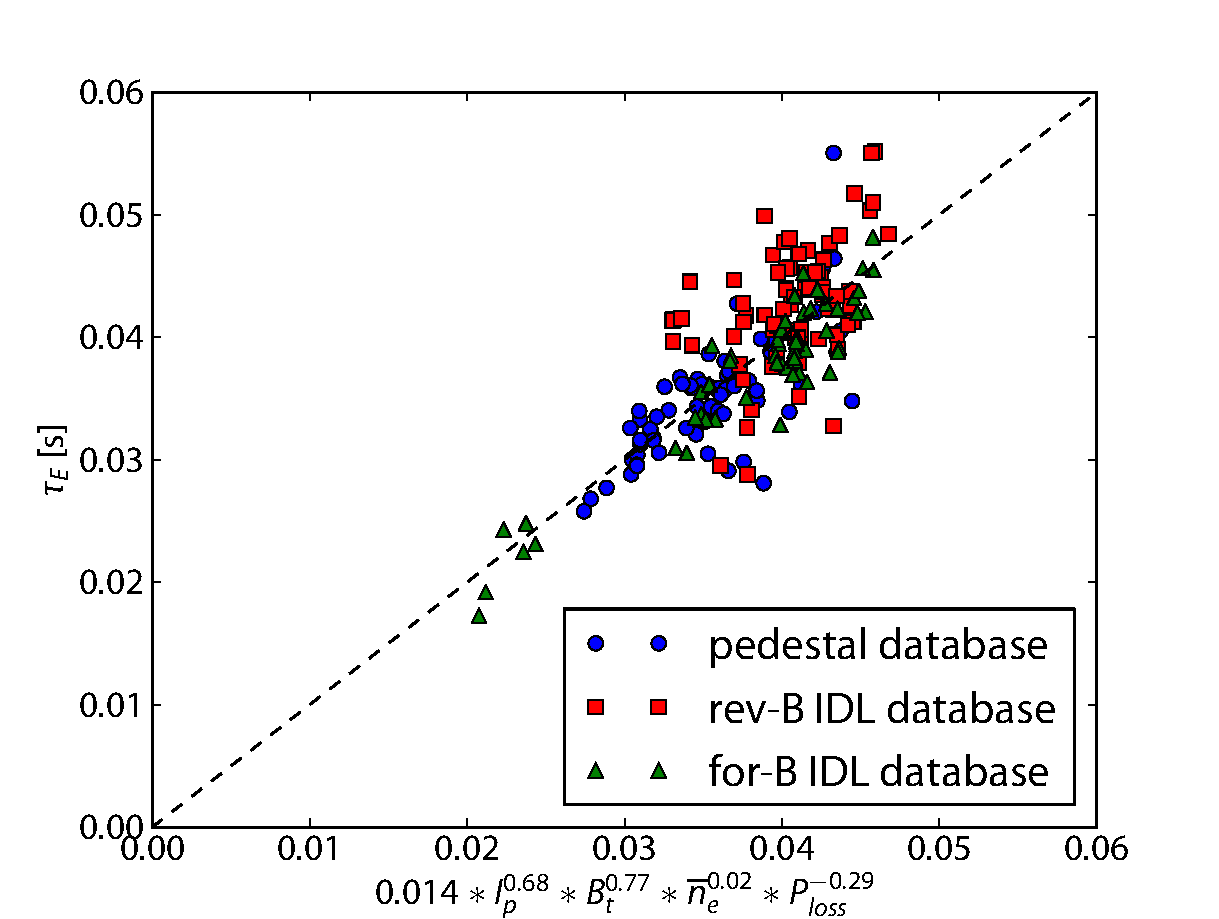
\includegraphics[width=100mm]{graphics/IModePedestal/tauE_3_Ploss_sep.pdf}}
\end{figure}

\begin{figure}
 \pushtooutside
 \fcapside[60mm]{\caption[Power-law fit to I-mode $\tau_E$, with fixed $R^2 \sqrt{\varepsilon}$ size scaling.]{Power-law fit to I-mode energy confinement time $\tau_E$, with the \emph{ansatz} of an $R^2 \sqrt{\varepsilon}$ size scaling fixed (fit \#5 in \cref{tab:imode_confinement}).  Both the high-resolution pedestal database and older reversed-field LSN and forward-field USN I-mode databases are used.  Note the expected weak degradation of $\tau_E$ with heating power.}\label{fig:imode_tauE_6}}{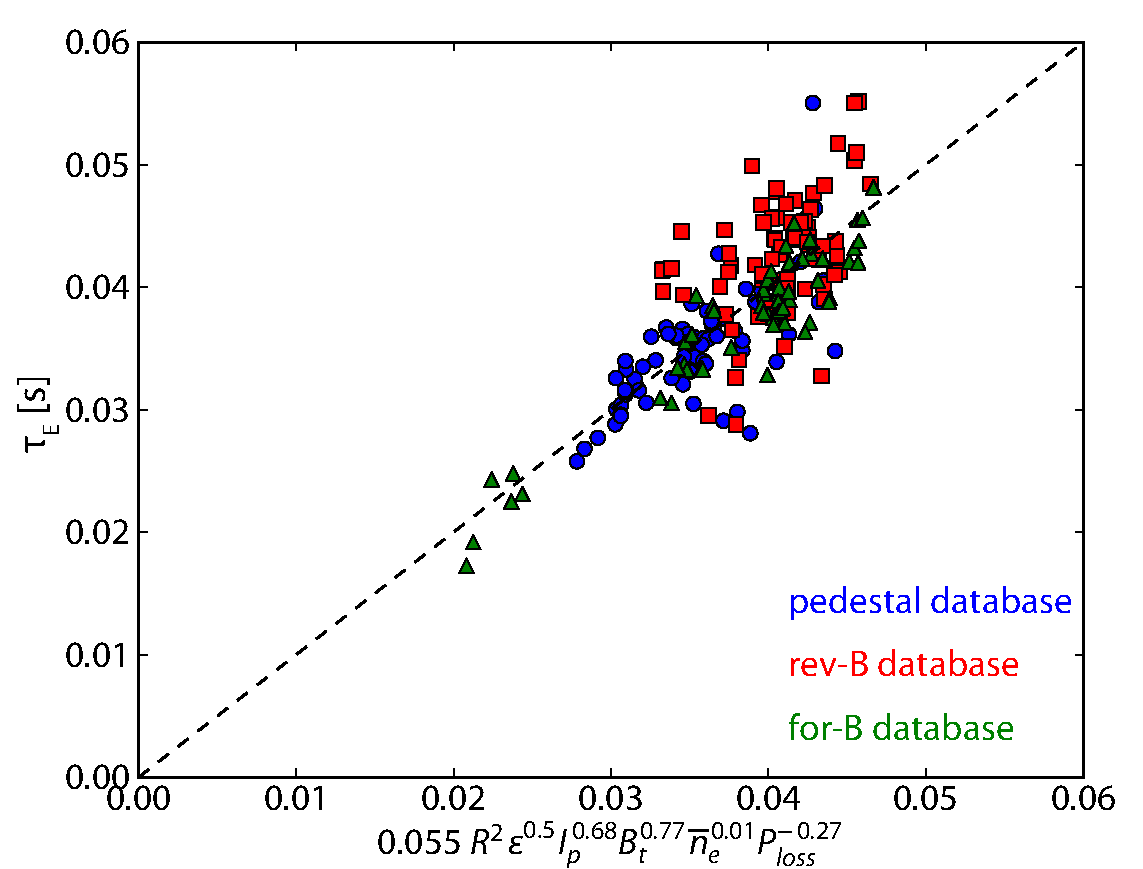
\includegraphics[width=100mm]{graphics/IModePedestal/tauE_6_Ploss_sep.pdf}}
\end{figure}

\begin{figure}
 \pushtooutside
 \fcapside[60mm]{\caption[Power-law fit to I-mode $\tau_E$ extrapolated to larger devices.]{Modeled energy confinement time $\tau_E$ with the fixed $R^2 \sqrt{\varepsilon}$ size scaling (fit \#5 in \cref{tab:imode_confinement}, extrapolated to DIII-D, ASDEX Upgrade, JET, and ITER.  Modeled energy confinement times are competitive with H-modes, both the measured $\tau_E$ for existing machines and the expected ITER98y2 prediction for ITER H-modes.}\label{fig:imode_tauE_extrap}}{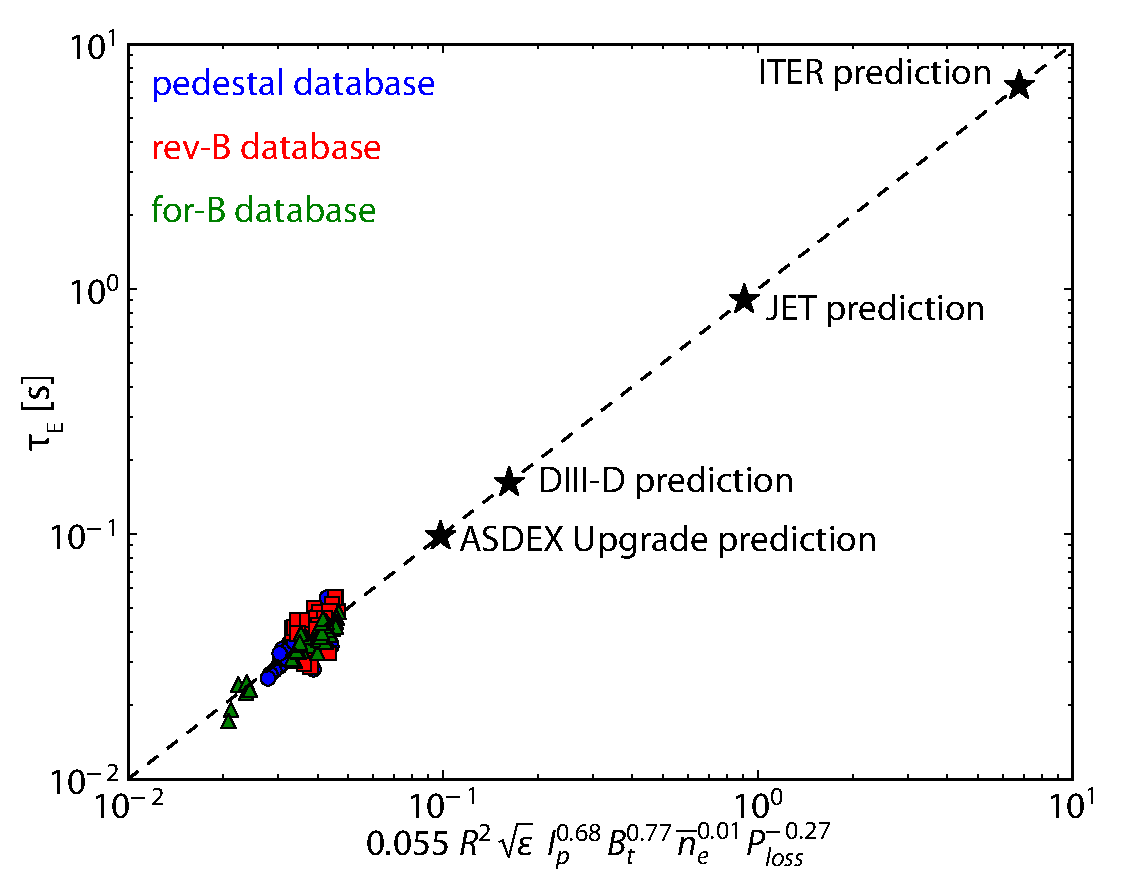
\includegraphics[width=100mm]{graphics/IModePedestal/tauE_6_Ploss_extrap.pdf}}
\end{figure}

\section{Fluctuation Characterization}\label{sec:imode_fluct}

\nicechapterending

\bibliographystyle{../plainurl}
\bibliography{../references}